% Copyright 2006 by Till Tantau
%
% This file may be distributed and/or modified
%
% 1. under the LaTeX Project Public License and/or
% 2. under the GNU Free Documentation License.
%
% See the file doc/generic/pgf/licenses/LICENSE for more details.


\section{Repeating Things: The Foreach Statement}
\label{section-foreach}

This section describes the package |pgffor|, which is loaded automatically by
\tikzname, but not by \pgfname:

\begin{package}{pgffor}
    This package can be used independently of \pgfname, but works particularly
    well together with \pgfname\ and \tikzname. It defines two new commands:
    |\foreach| and |\breakforeach|.
\end{package}

\begin{command}{\foreach| |\meta{variables}| |\opt{{\ttfamily[}\meta{options}{\ttfamily]}}| in |\meta{list}  \meta{commands}}
    The syntax of this command is a bit complicated, so let us go through it
    step-by-step.

    In the easiest case, \meta{variables} is a single \TeX-command like |\x| or
    |\point|. (If you want to have some fun, you can also use active
    characters. If you do not know what active characters are, you are
    blessed.)

    Still in the easiest case, \meta{options} will be omitted. The keys for
    customizing this command will be discussed below.

    Again, in the easiest case, \meta{list} is either a comma-separated list of
    values surrounded by curly braces or it is the name of a macro that contain
    such a list of values. Anything can be used as a value, but numbers are
    most likely.

    Finally, in the easiest case, \meta{commands} is some \TeX-text in curly
    braces.

    With all these assumptions, the |\foreach| statement will execute the
    \meta{commands} repeatedly, once for every element of the \meta{list}. Each
    time the \meta{commands} are executed, the \meta{variable} will be set to
    the current value of the list item.
    %
\begin{codeexample}[]
\foreach \x in {1,2,3,0} {[\x]}
\end{codeexample}

\begin{codeexample}[]
\def\mylist{1,2,3,0}
\foreach \x in \mylist {[\x]}
\end{codeexample}

    Note that in each execution of \meta{commands} the \meta{commands} are put
    in a \TeX\ group. This means that \emph{local changes to counters inside
    \meta{commands} do not persist till the next iteration}. For instance, if
    you add 1 to a counter inside \meta{commands} locally, then in the next
    iteration the counter will have the same value it had at the beginning of
    the first iteration. You have to add |\global| if you wish changes to
    persist from iteration to iteration.


    \medskip
    \textbf{Syntax for the commands.}
    Let us move on to a more complicated setting. The first complication occurs
    when the \meta{commands} are not some text in curly braces. If the
    |\foreach| statement does not encounter an opening brace, it will instead
    scan everything up to the next semicolon and use this as \meta{commands}.
    This is most useful in situations like the following:
    %
\begin{codeexample}[]
\tikz
  \foreach \x in {0,1,2,3}
    \draw (\x,0) circle (0.2cm);
\end{codeexample}

    However, the ``reading till the next semicolon'' is not the whole truth.
    There is another rule: If a |\foreach| statement is directly followed by
    another |\foreach| statement, this second foreach statement is collected as
    \meta{commands}. This allows you to write the following:
    %
\begin{codeexample}[]
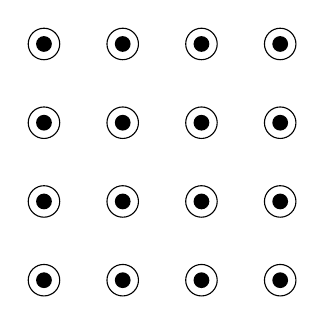
\begin{tikzpicture}
  \foreach \x in {0,1,2,3}
    \foreach \y in {0,1,2,3}
      {
        \draw (\x,\y) circle (0.2cm);
        \fill (\x,\y) circle (0.1cm);
      }
\end{tikzpicture}
\end{codeexample}

    \medskip
    \textbf{The dots notation.}
    The second complication concerns the \meta{list}. If this \meta{list}
    contains the list item ``|...|'', this list item is replaced by the
    ``missing values''. More precisely, the following happens:

    Normally, when a list item |...| is encountered, there should already have
    been \emph{two} list items before it, which where numbers. Examples of
    \emph{numbers} are |1|, |-10|, or |-0.24|. Let us call these numbers $x$
    and $y$ and let $d := y-x$ be their difference. Next, there should also be
    one number following the three dots, let us call this number~$z$.

    In this situation, the part of the list reading ``$x$|,|$y$|,...,|$z$'' is
    replaced by ``$x$, $x+d$, $x+2d$, $x+3d$, \dots, $x+md$'', where the last
    dots are semantic dots, not syntactic dots. The value $m$ is the largest
    number such that $x + md \le z$ if $d$ is positive or such that $x+md \ge
    z$ if $d$ is negative.

    Perhaps it is best to explain this by some examples:  The following
    \meta{list} have the same effects:

    |\foreach \x in {1,2,...,6} {\x, }| yields \foreach \x in {1,2,...,6} {\x, }

    |\foreach \x in {1,2,3,...,6} {\x, }| yields \foreach \x in {1,2,3,...,6} {\x, }

    |\foreach \x in {1,3,...,11} {\x, }| yields \foreach \x in {1,3,...,11} {\x, }

    |\foreach \x in {1,3,...,10} {\x, }| yields \foreach \x in {1,3,...,10} {\x, }

    |\foreach \x in {0,0.1,...,0.5} {\x, }| yields \foreach \x in {0,0.1,...,0.5} {\x, }

    |\foreach \x in {a,b,9,8,...,1,2,2.125,...,2.5} {\x, }| yields \foreach \x in {a,b,9,8,...,1,2,2.125,...,2.5} {\x, }

    As can be seen, for fractional steps that are not multiples of $2^{-n}$ for
    some small $n$, rounding errors can occur pretty easily. Thus, in the
    second last case, |0.5| should probably be replaced by |0.501| for
    robustness.

    There is another special case for the |...| statement: If the |...| is used
    right after the first item in the list, that is, if there is an $x$, but no
    $y$, the difference $d$ obviously cannot be computed and is set to $1$ if
    the number $z$ following the dots is larger than $x$ and is set to $-1$ if
    $z$ is smaller:

    |\foreach \x in {1,...,6} {\x, }| yields \foreach \x in {1,...,6} {\x, }

    |\foreach \x in {9,...,3.5} {\x, }| yields \foreach \x in {9,...,3.5} {\x, }

    There is a yet another special case for the |...| statement, in that it can
    indicate an alphabetic character sequence:

    |\foreach \x in {a,...,m} {\x, }| yields \foreach \x in {a,...,m} {\x, }

    |\foreach \x in {Z,X,...,M} {\x, }| yields \foreach \x in {Z,X,...,M} {\x, }

    A final special case for the |...| statement is contextual replacement. If
    the |...| is used in some context, for example, |sin(...)|, this context
    will be interpreted correctly, provided that the list items prior to the
    |...| statement have \emph{exactly} the same pattern, except that, instead
    of dots, they have a number or a character:

    |\foreach \x in {2^1,2^...,2^7} {$\x$, }| yields \foreach \x in {2^1,2^...,2^7} {$\x$, }

    |\foreach \x in {0\pi,0.5\pi,...\pi,3\pi} {$\x$, }| yields \foreach \x in {0\pi,0.5\pi,...\pi,3\pi} {$\x$, }

    |\foreach \x in {A_1,..._1,H_1} {$\x$, }| yields \foreach \x in {A_1,..._1,H_1} {$\x$, }


    \textbf{Special handling of pairs.}
    Different list items are separated by commas. However, this causes a
    problem when the list items contain commas themselves as pairs like |(0,1)|
    do. In this case, you should put the items containing commas in braces as
    in |{(0,1)}|. However, since pairs are such a natural and useful case, they
    get a special treatment by the |\foreach| statement. When a list item
    starts with a |(| everything up to the next |)| is made part of the item.
    Thus, we can write things like the following:
    %
\begin{codeexample}[]
\tikz
  \foreach \position in {(0,0), (1,1), (2,0), (3,1)}
    \draw \position rectangle +(.25,.5);
\end{codeexample}


    \medskip
    \textbf{Using the foreach-statement inside paths.}
    \tikzname\ allows you to use |foreach| and |\foreach| (both have the same
    effect) inside a path construction. In such a case, the \meta{commands}
    must be path construction commands. Here are two examples:
    %
\begin{codeexample}[]
\tikz
  \draw (0,0)
    foreach \x in {1,...,3}
      { -- (\x,1) -- (\x,0) }
    ;
\end{codeexample}

\begin{codeexample}[]
\tikz \draw foreach \p in {1,...,3} {(\p,1)--(\p,3) (1,\p)--(3,\p)};
\end{codeexample}

    Note that the |node| and |pic| path commands also support the |foreach|
    statement in special ways.


    \medskip
    \textbf{Multiple variables.}
    You will often wish to iterate over two variables at the same time. Since
    you can nest |\foreach| loops, this is normally straight-forward. However,
    you sometimes wish variables to iterate ``simultaneously''. For example, we
    might be given a list of edges that connect two coordinates and might wish
    to iterate over these edges. While doing so, we would like the source and
    target of the edges to be set to two different variables.

    To achieve this, you can use the following syntax: The \meta{variables} may
    not only be a single \TeX-variable. Instead, it can also be a list of
    variables separated by slashes (|/|). In this case the list items can also
    be lists of values separated by slashes.

    Assuming that the \meta{variables} and the list items are lists of values,
    each time the \meta{commands} are executed, each of the variables in
    \meta{variables} is set to one part of the list making up the current list
    item. Here is an example to clarify this:

    \example |\foreach \x / \y in {1/2,a/b} {``\x\ and \y''}| yields
    \foreach \x / \y in {1/2,a/b} {``\x\ and \y''}.

    If some entry in the \meta{list} does not have ``enough'' slashes, the last
    entry will be repeated. Here is an example:
    %
\begin{codeexample}[]
\begin{tikzpicture}
  \foreach \x/\xtext in {0,...,3,2.72 / e}
    \draw (\x,0) node{$\xtext$};
\end{tikzpicture}
\end{codeexample}

    Here are more useful examples:
    %
\begin{codeexample}[]
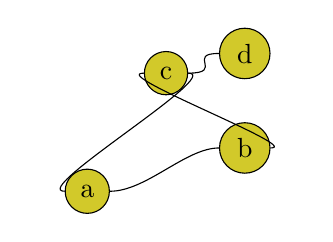
\begin{tikzpicture}
  % Define some coordinates:
  \path[nodes={circle,fill=yellow!80!black,draw}]
    (0,0)    node(a) {a}
    (2,0.55) node(b) {b}
    (1,1.5)  node(c) {c}
    (2,1.75) node(d) {d};

  % Draw some connections:
  \foreach \source/\target in {a/b, b/c, c/a, c/d}
    \draw (\source) .. controls +(.75cm,0pt) and +(-.75cm,0pt)..(\target);
\end{tikzpicture}
\end{codeexample}

\begin{codeexample}[]
\begin{tikzpicture}
  % Let's draw circles at interesting points:
  \foreach \x / \y / \diameter in {0 / 0 / 2mm, 1 / 1 / 3mm, 2 / 0 / 1mm}
    \draw (\x,\y) circle (\diameter);

  % Same effect
  \foreach \center/\diameter in {{(0,0)/2mm}, {(1,1)/3mm}, {(2,0)/1mm}}
    \draw[yshift=2.5cm] \center circle (\diameter);
\end{tikzpicture}
\end{codeexample}

\begin{codeexample}[]
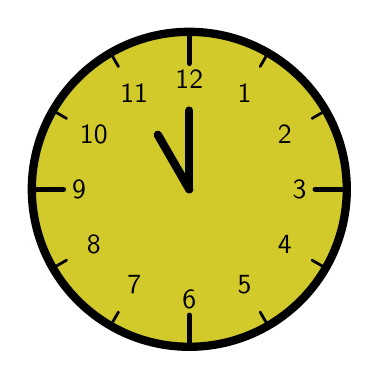
\begin{tikzpicture}[line cap=round,line width=3pt]
  \filldraw [fill=yellow!80!black] (0,0) circle (2cm);

  \foreach \angle / \label in
    {0/3, 30/2, 60/1, 90/12, 120/11, 150/10, 180/9,
     210/8, 240/7, 270/6, 300/5, 330/4}
  {
    \draw[line width=1pt] (\angle:1.8cm) -- (\angle:2cm);
    \draw (\angle:1.4cm) node{\textsf{\label}};
  }

  \foreach \angle in {0,90,180,270}
    \draw[line width=2pt] (\angle:1.6cm) -- (\angle:2cm);

  \draw (0,0) -- (120:0.8cm); % hour
  \draw (0,0) -- (90:1cm);    % minute
\end{tikzpicture}%
\end{codeexample}

\begin{codeexample}[]
\tikz[shading=ball]
  \foreach \x / \cola in {0/red,1/green,2/blue,3/yellow}
    \foreach \y / \colb in {0/red,1/green,2/blue,3/yellow}
      \shade[ball color=\cola!50!\colb] (\x,\y) circle (0.4cm);
\end{codeexample}


    \medskip
    \textbf{Options to customize the foreach-statement.}

    The keys described below can be used in the \meta{options} argument to the
    |\foreach| command. They all have the path |/pgf/foreach/|, however, the
    path is set automatically when \meta{options} are parsed, so it does not
    have to be explicitly stated.

    \begin{key}{/pgf/foreach/var=\meta{variable}}
        This key provides an alternative way to specify variables:
        |\foreach [var=\x,var=\y]| is the same as |\foreach \x/\y|. If used,
        this key should be used before the other keys.
    \end{key}

    \begin{key}{/pgf/foreach/evaluate=\meta{variable}| |\opt{|as |\meta{macro}| using |\meta{formula}}}
        By default, list items are not evaluated: |1+2|, yields |1+2|, not |3|.
        This key allows a variable to be evaluated using the mathematical
        engine. The variable must have been specified either using the |var|
        key or in the \meta{variables} argument of the |foreach| command. By
        default, the result of the evaluation will be stored in
        \meta{variable}. However, the optional |as |\meta{macro} statement can
        be used to store the result in \meta{macro}.
        %
\begin{codeexample}[]
\foreach \x [evaluate=\x] in {2^0,2^...,2^8}{$\x$, }
\end{codeexample}

\begin{codeexample}[]
\foreach \x [evaluate=\x as \xeval] in {2^0,2^...,2^8}{$\x=\xeval$, }
\end{codeexample}

        The optional |using |\meta{formula} statement means an evaluation does
        not have to be explicitly stated for each item in \meta{list}. The
        \meta{formula} should contain at least one reference to
        \meta{variable}.
        %
\begin{codeexample}[]
\tikz\foreach \x [evaluate=\x as \shade using \x*10] in {0,1,...,10}
  \node [fill=red!\shade!yellow, minimum size=0.65cm] at (\x,0) {\x};
\end{codeexample}
        %
    \end{key}

    \begin{key}{/pgf/foreach/remember=\meta{variable}| as |\meta{macro}| |\opt{|(initially |\meta{value}|)|}}
        This key allows the item value stored in \meta{variable} to be
        remembered during the next iteration, stored in \meta{macro}. If a
        variable is evaluated, the result of this evaluation is remembered. By
        default the value of \meta{variable} is zero for the first iteration,
        however, the optional |(initially |\meta{value}|)| statement, allows
        the \meta{macro} to be initially defined as \meta{value}.
        %
\begin{codeexample}[]
\foreach \x [remember=\x as \lastx (initially A)] in {B,...,H}{$\overrightarrow{\lastx\x}$, }
\end{codeexample}
        %
    \end{key}

    \begin{key}{/pgf/foreach/count=\meta{macro}| |\opt{|from |\meta{value}}}
        This key allows \meta{macro} to hold the position in the list of the
        current item. The optional |from |\meta{value} statement allows the
        counting to begin from \meta{value}.
        %
\begin{codeexample}[]
\tikz[x=0.75cm,y=0.75cm]
  \foreach \x [count=\xi] in {a,...,e}
    \foreach \y [count=\yi] in {\x,...,e}
      \node [draw, top color=white, bottom color=blue!50, minimum size=0.666cm]
        at (\xi,-\yi) {$\mathstrut\x\y$};
\end{codeexample}
        %
    \end{key}

    \begin{key}{/pgf/foreach/parse=\marg{boolean} (default false)}
        If this key is set to true the upper bound in the loop will be
        fed into |\pgfmathparse|. This allows to use complex expressions as
        the upper bound. However, the expression must be safe for evaluation
        in |\pgfmathparse|. It is known that internal \TeX\ registers can
        cause trouble.
        %
\begin{codeexample}[]
\foreach \x [parse=true] in {1,...,1.0e+1 - 1}{ \x }
\end{codeexample}
        %
    \end{key}
\end{command}

\begin{command}{\breakforeach}
    If this command is given inside a |\foreach| command, no further executions
    of the \meta{commands} will occur. However, the current execution of the
    \meta{commands} is continued normally, so it is probably best to use this
    command only at the end of a |\foreach| command.
    %
\begin{codeexample}[]
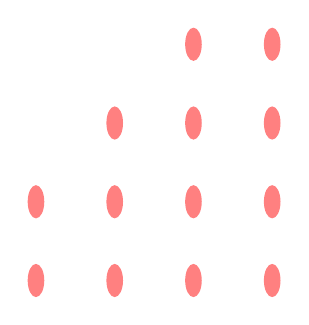
\begin{tikzpicture}
  \foreach \x in {1,...,4}
    \foreach \y in {1,...,4}
    {
      \fill[red!50] (\x,\y) ellipse (3pt and 6pt);

      \ifnum \x<\y
        \breakforeach
      \fi
    }
\end{tikzpicture}
\end{codeexample}
    %
\end{command}
